%!TEX root = ../../book_ML.tex
\chapter{Máy vector hỗ trợ lề mềm}
% \chapter{Soft-margin support vector machine}
 
\index{SVM lề mềm -- soft-margin SVM}
 
\section{Giới thiệu}
Giống với thuật toán học perceptron (PLA), máy vector hỗ trợ (SVM) chỉ làm việc khi dữ liệu của hai lớp tách biệt tuyến tính. Một cách tự nhiên, chúng ta cũng mong muốn SVM có thể làm việc với dữ liệu gần tách btệt tuyến tính như hồi quy logistic đã làm được.  
 
% \textit{Bạn được khuyến khích đọc bài \href{http://machinelearningcoban.com(/2017/04/09/smv/}{Support Vector Machine}) trước khi đọc bài này.} 
 

 
% <hr> 
% <div> 
% <table width = "100%" style = "border: 0px solid white; align = center"> 
%    <tr > 
%         <td width="40%" style = "border: 0px solid white" align = "center"> 
%         <img style="display:block;" width = "100%" src = "/assets/20_softmarginsvm/ssvm1.png"> 
%         <br> 
%         a) 
%          </td> 
 
%         <td width="40%" style = "border: 0px solid white" align = "center"> 
%         <img style="display:block;" width = "100%" src = "/assets/20_softmarginsvm/ssvm2.png"> 
%         <br> 
%         b) 
%         </td> 
 
%     </tr> 
 
% </table> 
% <div class = "thecap"> Hình 1: Soft margin SVM. Khi a) có nhiễu hoặc b) dữ liệu gần linearly separable, SVM thuần sẽ không hoạt động hiệu quả. 
% </div> 
% </div> 
% <hr> 
 

\begin{figure}[t]
    \begin{subfigure}{0.46\textwidth}
    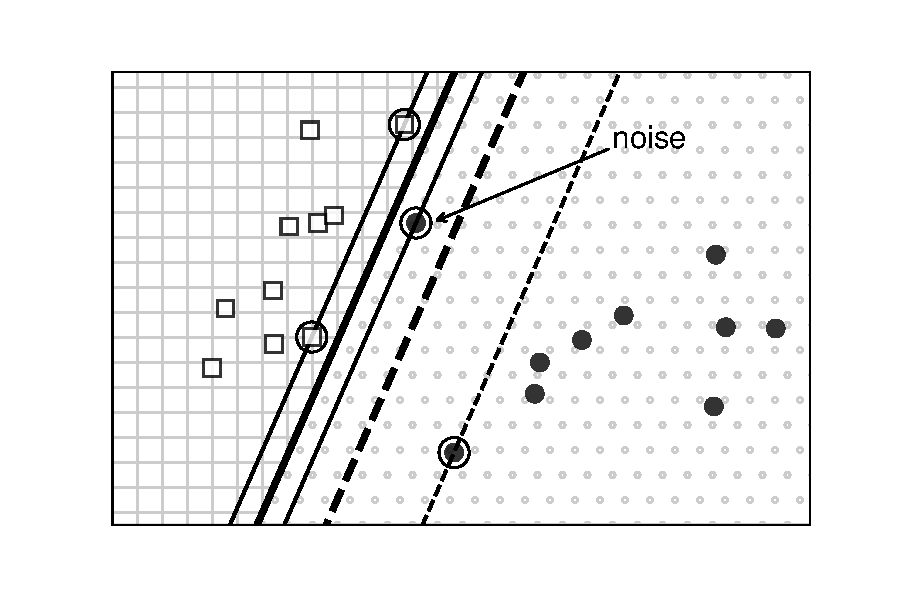
\includegraphics[width=0.95\linewidth]{ebookML_src/src/softmargin_svm/ssvm1.pdf}
    \caption{Khi có nhiễu nhỏ.}
    \label{fig:20_1a}
    \end{subfigure}
    \begin{subfigure}{0.48\textwidth}
    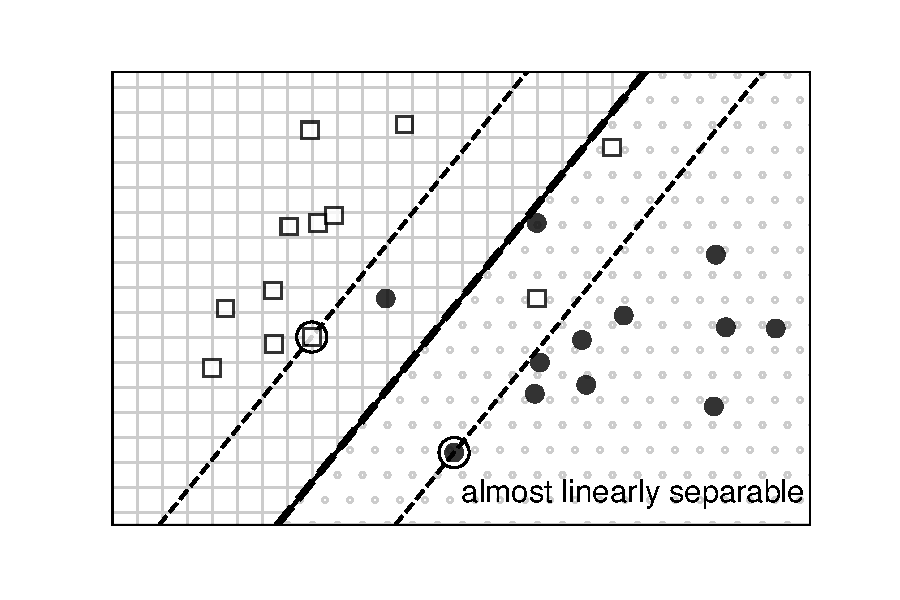
\includegraphics[width=0.95\linewidth]{ebookML_src/src/softmargin_svm/ssvm2.pdf}
    \caption{Khi dữ liệu \textit{gần linearly separable}.}
    \label{fig:20_1b}
    \end{subfigure}
    \caption{Hai trường hơp khi SVM \textit{thuần} làm việc không hiệu quả. (a) Hai lớp vẫn tách biệt tuyến tính nhưng một điểm thuộc lớp này quá gần lớp kia, điểm này có thể là nhiễu. (b) Dữ liệu hai lớp gần tách biệt tuyến tính.}
    \label{fig:20_1}
\end{figure}


Xét hai ví dụ trong Hình~\ref{fig:20_1}. Có hai trường hợp dễ nhận thấy SVM làm
việc không hiệu quả hoặc thậm chí không làm việc: 

\begin{itemize}
    \item Trường hợp 1: Dữ liệu vẫn tách biệt tuyến tính như Hình~\ref{fig:20_1a}
    nhưng có một điểm nhiễu của lớp tròn ở quá gần lớp vuông. Trong
    trường hợp này, SVM sẽ tạo ra lề rất nhỏ. Ngoài ra, mặt phân cách nằm quá gần các điểm
    vuông và xa các điểm tròn. Trong khi đó, nếu \textit{hy sinh} điểm
    nhiễu này thì ta thu được nghiệm là đường nét đứt đậm. Nghiệm này tạo ra lề rộng hơn, có khả năng tăng độ chính xác cho mô hình. 
     
    \item Trường hợp 2: Dữ liệu gần tách biệt tuyến tính như trong Hình~\ref{fig:20_1b}. Trong trường hợp
    này, không tồn tại đường thẳng nào hoàn toàn phân chia hai lớp dữ liệu, vì
    vậy bài toán tối ưu SVM vô nghiệm. Tuy nhiên, nếu chấp nhận việc những điểm ở gần khu vực ranh giới bị phân loại lỗi, ta vẫn có
    thể tạo được một đường phân chia khá tốt như đường nét đứt đậm. Các
    đường hỗ trợ (nét đứt mảnh) vẫn giúp tạo được lề lớn. Với mỗi điểm nằm \textit{lần} sang
    phía bên kia của các đường hỗ trợ tương ứng, ta gọi điểm đó rơi vào
    \textit{vùng không an toàn}. Như trong hình, hai điểm tròn nằm phía bên
    trái đường hỗ trợ của lớp tròn được xếp vào loại không an toàn, mặc
    dù có một điểm tròn vẫn nằm trong khu vực nền chấm. Hai điểm vuông ở
    phía phải của đường hỗ trợ của lớp tương ứng thậm chí đều lấn sang phần
    có nền chấm. 
\end{itemize}
\index{SVM lề mềm -- soft-margin SVM}
\index{SVM lề cứng -- hard-margin SVM}
Trong cả hai trường hợp trên, lề tạo bởi đường phân chia và đường
nét đứt mảnh được gọi là \textit{lề mềm} ({soft-margin}). Từ \textit{mềm} thể hiện sự linh hoạt, có thể chấp nhận việc một vài điểm bị phân loại sai để mô hình hoạt động tốt hơn trên toàn bộ dữ liệu. SVM tạo ra các lề mềm được gọi là \textit{SVM lề mềm} (soft-margin SVM). Để phân
biệt, SVM \textit{thuần} trong chương trước được gọi là SVM lề cứng (hard-margin SVM).
 
Có hai cách xây dựng và giải quyết bài toán tối ưu SVM lề mềm. Cả hai đều mang lại những kết quả thú vị, có thể phát triển tiếp thành các
thuật toán SVM phức tạp và hiệu quả hơn như sẽ thấy trong các chương sau. Cách thứ nhất là giải một bài toán tối ưu có ràng buộc thông qua việc giải bài
toán đối ngẫu như với SVM lề cứng. Hướng giải quyết này là cơ sở cho phương pháp \textit{SVM hạt nhân} áp dụng cho dữ liệu không thực
sự tách biệt tuyến tính được đề cập trong chương tiếp theo. Cách
giải quyết thứ hai là đưa về một bài toán tối ưu không ràng buộc, giải được bằng các phương pháp gradient descent. Nhờ đó, hướng giải
quyết này có thể được áp dụng cho các bài toán quy mô lớn. Ngoài ra, trong cách
giải này, chúng ta sẽ làm quen với một hàm mất mát mới có tên là \textit{bản lề} (hinge). Hàm mất mát này có thể được mở rộng cho bài toán phân loại đa lớp được đề cập trong chương~\ref{cha:multisvm}. Cách phát triển
từ SVM lề mềm thành SVM đa lớp có thể được so sánh
với cách phát triển từ hồi quy logistic thành hồi quy softmax. 
 
% Hướng giải quyết này sẽ được tôi trình bày trong Mục 3 bên dưới.
 
 
\section{Phân tích toán học}
 
Như đã đề cập phía trên, để có một lề rộng hơn trong SVM lề mềm, ta cần {hy sinh} một vài điểm dữ liệu bằng cách chấp nhận
cho chúng rơi vào vùng {không an toàn}. Tất nhiên, việc {hy sinh}
này cần được hạn chế; nếu không, ta có thể tạo ra một biên cực lớn bằng cách
{hy sinh} hầu hết các điểm. Vậy hàm mục tiêu nên là một sự kết hợp sao cho lề được tối đa và sự hy sinh được tối thiểu.
 
% ******************************************************************************
\begin{figure}[t]
    % caption on side     
    \floatbox[{\capbeside\thisfloatsetup{capbesideposition={right,top},capbesidewidth=6cm}}]{figure}[\FBwidth]
    {\caption{ 
    Giới thiệu các biến lỏng lẻo $\xi_n$. Với các điểm nằm trong {khu vực an
    toàn}, $\xi_n = 0$.
    Những điểm nằm trong vùng
    không an toàn nhưng vẫn đúng phía so với đường ranh giới (đường nét đứt
    đậm) tương ứng với các $0 < \xi_n < 1$, ví dụ $\mathbf{x}_2$. Những điểm
    nằm ngược phía lớp thực sự của chúng so với đường nét đứt đậm tương ứng $\xi_n > 1$, ví dụ như $\mathbf{x}_1$ và $\mathbf{x}_3$.
    }
    \label{fig:20_2}}
    { % figure here
    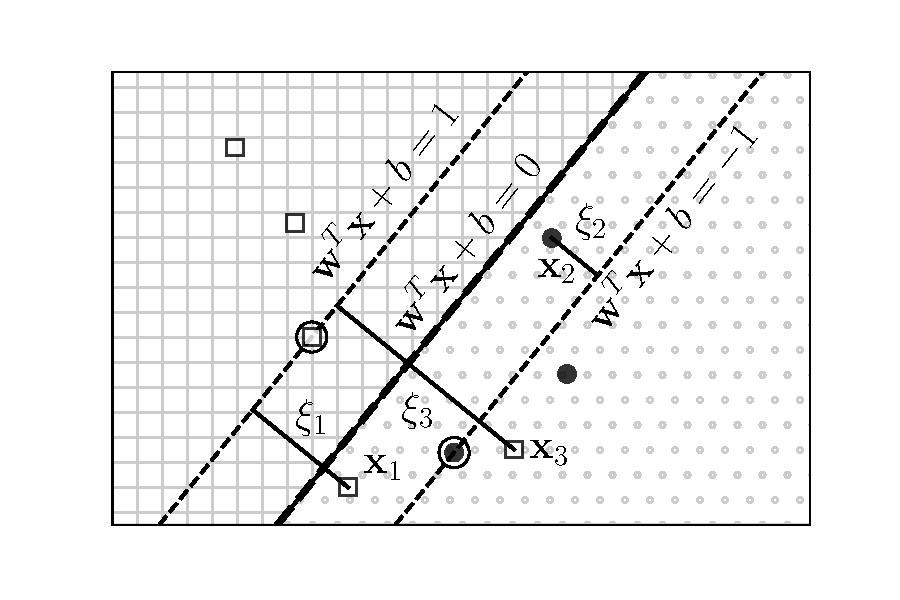
\includegraphics[width=.55\textwidth]{ebookML_src/src/softmargin_svm/ssvm3.pdf}
    }
    % \myrule
\end{figure}
% ******************************************************************************
\index{biến lỏng lẻo -- slack variable}
Giống SVM lề cứng, việc tối đa lề có thể đưa
về việc tối thiểu $\|\mathbf{w}\|_2^2$. Để đong đếm sự hy sinh, chúng ta cùng quan sát Hình~\ref{fig:20_2}. Với mỗi điểm $\mathbf{x}_n$ trong tập huấn luyện, ta \textit{giới thiệu} thêm một biến đo \textit{sự hy
sinh} $\xi_n$ tương ứng. Biến này còn được gọi là \textit{biến lỏng lẻo} (slack variable). Với
những điểm $\mathbf{x}_n$ nằm trong {vùng an toàn} (nằm đúng vào màu nền
tương ứng và nằm ngoài khu vực lề), $\xi_n = 0$, tức không có sự
{hy sinh} nào xảy ra. Với mỗi điểm nằm trong {vùng không
an toàn} như $\mathbf{x}_1,
\mathbf{x}_2$ hay $\mathbf{x}_3$ ta cần có $\xi_i > 0$ để đo sự hy sinh. Đại lượng này cần tỉ lệ với khoảng cách từ vị trí vi phạm tương ứng tới
biên giới an toàn (đường nét đứt mảnh tương ứng với lớp đó). Nhận thấy nếu $y_i= \pm 1$ là {nhãn} của
$\mathbf{x}_i$ trong {vùng không an toàn} thì $\xi_i$ có thể được định
nghĩa bởi
\begin{equation}
    \xi_i = |\mathbf{w}^T\mathbf{x}_i + b - y_i|
\end{equation}
(Mẫu số $\|\bw\|_2$ được lược bỏ vì ta chỉ cần một đại lượng tỉ lệ thuận.)
Nhắc lại bài toán tối ưu cho SVM lề cứng: 
\begin{eqnarray}  
\label{eqn:20_1}
\begin{aligned}
    (\mathbf{w}, b) &= \arg \min_{\mathbf{w}, b} \frac{1}{2}{\|\mathbf{w}\|_2^2}   \\\ 
    \text{thoả mãn:}~ & y_n(\mathbf{w}^T\mathbf{x}_n + b) \geq 1, ~~\forall n = 1, 2, \dots, N 
\end{aligned}
\end{eqnarray} 
Với SVM lề mềm, hàm mục tiêu sẽ có thêm một số hạng nữa giúp tối
thiểu {tổng sự hy sinh}. Từ đó ta có hàm mục tiêu:
\begin{equation} 
\frac{1}{2}{\|\mathbf{w}\|_2^2} + C \sum_{n=1}^N \xi_n 
\end{equation} 
trong đó $C$ là một hằng số dương. Hằng số $C$ được dùng để điều chỉnh tầm quan trọng giữa độ rộng lề và
sự hy sinh. 
% Nếu $C$ quá nhỏ, sự hy sinh không còn được coi
% trọng, nghiệm tìm được sẽ tạo ra biên rất lớn, nhưng cũng có rất nhiều điểm bị phân lớp sai. Nếu $C$ quá lớn,
% lề không còn được coi trọng, ta có thể giảm thiểu sự
% hy sinh nhưng lề tạo được sẽ rất nhỏ. Việc tìm $C$ có thể được thực hiện thông qua xác thực chéo.
% \newpage  

Điều kiện ràng buộc cũng được thay đổi so với SVM lề cứng. Với mỗi cặp dữ liệu $(\mathbf{x}_n,
y_n)$, thay vì ràng buộc {cứng} $y_n(\mathbf{w}^T\mathbf{x}_n + b) \geq
1$, ta sử dụng ràng buộc {mềm}:  
\begin{equation*} 
y_n(\mathbf{w}^T\mathbf{x}_n + b) \geq 1 - \xi_n \Leftrightarrow 1 - \xi_n - y_n(\mathbf{w}^T\mathbf{x}_n + b) \leq 0, ~~ \forall n = 1, 2, \dots, n 
\end{equation*} 
Và ràng buộc phụ $\xi_n \geq 0, ~\forall n = 1, 2, \dots, N$. 
% \newpage  
Tóm lại, ta có bài toán tối ưu chính cho SVM lề mềm
như sau: 
\begin{eqnarray}  
\label{eqn:20_2}
\begin{aligned}
    (\mathbf{w}, b, \xi) &= \arg \min_{\mathbf{w}, b, \xi} \frac{1}{2}{\|\mathbf{w}\|_2^2} + C \sum_{n=1}^N \xi_n  \\\ 
    \text{thoả mãn:}~ & 1 - \xi_n - y_n(\mathbf{w}^T\mathbf{x}_n + b) \leq 0, \forall n = 1, 2, \dots, N  \\\ 
    & -\xi_n \leq 0,  ~\forall n = 1, 2, \dots, N 
\end{aligned}
\end{eqnarray} 
 
 
\textit{Nhận xét:} 
\begin{itemize}
    \item Nếu $C$ nhỏ, việc {sự hy sinh} cao hay thấp không gây ảnh hưởng
    nhiều tới giá trị của hàm mục tiêu, thuật toán sẽ điều chỉnh sao cho
    $\|\mathbf{w}\|_2^2$ nhỏ nhất, tức lề lớn nhất, điều này
    dẫn tới $\sum_{n=1}^N\xi_n$ sẽ lớn theo vì vùng an toàn bị nhỏ đi. Ngược
    lại, nếu $C$ quá lớn, để hàm mục tiêu đạt giá trị nhỏ nhất, thuật toán sẽ
    tập trung vào làm giảm $\sum_{n=1}^N\xi_n$. Trong trường hợp $C$ rất rất lớn
    và hai lớp dữ liệu tách biệt tuyến tính, ta sẽ thu được $\sum_{n=1}^N\xi_n
    = 0$. Điều này đồng nghĩa với
    việc không có điểm nào phải {hy sinh}, nghiệm thu được cũng chính là nghiệm của SVM lề cứng. Nói cách khác, SVM lề cứng là
    một trường hợp đặc biệt của SVM lề mềm.
     
    \item Bài toán tối ưu \eqref{eqn:20_2} có thêm sự xuất hiện của các
    biến lỏng lẻo $\xi_n$. Các $\xi_n = 0$ ứng với những
    điểm dữ liệu nằm trong {vùng an toàn}. Các $0 < \xi_n \leq 1$ ứng với những điểm nằm trong {vùng không an toàn} nhưng vẫn được phân
    loại
    đúng, tức vẫn nằm về đúng phía so với đường phân chia. Các $\xi_n > 1$
    tương ứng với các điểm bị phân loại sai.
     
    \item Hàm mục tiêu trong bài toán tối ưu \eqref{eqn:20_2} là một hàm lồi vì nó là tổng của hai hàm lồi: một hàm chuẩn và một hàm tuyến tính. Các hàm ràng buộc cũng là các hàm tuyến tính theo $(\mathbf{w}, b, \xi)$. Vì vậy bài toán tối ưu \eqref{eqn:20_2} là một bài toán lồi, hơn nữa còn có thể biểu diễn dưới dạng một bài toán quy hoạch toàn phương.  
\end{itemize}
 
Tiếp theo, chúng ta sẽ giải bài toán tối ưu \eqref{eqn:20_2} bằng hai
cách khác nhau. 
% Cách thứ nhất thông qua giải bài toán đối ngẫu, cách thứ hai
% đưa
% \tcr{stop here}
 
\section{Bài toán đối ngẫu Lagrange }
Lưu ý rằng bài toán này có thể giải trực tiếp bằng các công cụ hỗ trợ quy hoạch toàn phương, nhưng
giống như với SVM lề cứng, chúng ta sẽ quan tâm hơn tới bài toán đối ngẫu của nó. 
 
Trước kết, ta cần kiểm tra tiêu chuẩn Slater của bài toán tối ưu lồi
\eqref{eqn:20_2}. Nếu tiêu chuẩn này thoả mãn, đối ngẫu mạnh sẽ
thoả mãn, và ta có thể tìm nghiệm của bài toán tối ưu~\eqref{eqn:20_2} thông qua
hệ điều kiện KKT (xem Chương~\ref{cha:duality}). 
 
 
\subsection{Kiểm tra tiêu chuẩn Slater}
 
Rõ ràng là với mọi $n = 1, 2, \dots, N$ và $(\mathbf{w}, b)$, ta luôn có thể tìm được các số {dương} $\xi_n, n = 1, 2, \dots, N,$ đủ lớn sao cho
\begin{math} 
y_n(\mathbf{w}^T\mathbf{x}_n + b) + \xi_n > 1, ~\forall n = 1, 2, \dots, N 
\end{math}.
Vì vậy, tồn tại điểm khả thi chặt cho bài toán và tiêu chuẩn Slater thỏa mãn. 
 
 
\subsection{Hàm Lagrange của bài toán SVM lề mềm}
Hàm Lagrange cho bài toán~\eqref{eqn:20_2} là
\begin{equation} 
\label{eqn:20_3}
\mathcal{L}(\mathbf{w}, b, \bxi, \blambda, \bmu) =
\frac{1}{2}{\|\mathbf{w}\|_2^2} + C \sum_{n=1}^N \xi_n + \sum_{n=1}^N \lambda_n ( 1 - \xi_n - y_n(\mathbf{w}^T\mathbf{x}_n + b)) - \sum_{n=1}^N \mu_n \xi_n
\end{equation} 
với $\blambda = [\lambda_1, \lambda_2, \dots, \lambda_N]^T \succeq 0$ và $\bmu =
[\mu_1, \mu_2, \dots, \mu_N]^T \succeq 0$ là các biến đối ngẫu Lagrange.
 % (vector nhân tử Lagrange). 
 
 
\subsection{Bài toán đối ngẫu }
 
Hàm số đối ngẫu của bài toán tối ưu \eqref{eqn:20_2} là: 
\begin{equation*} 
% \label{eqn:20_lagrangian}
g(\blambda, \bmu) = \min_{\mathbf{w}, b, \bxi} \mathcal{L}(\mathbf{w}, b, \bxi,
\blambda, \bmu) 
\end{equation*} 
Với mỗi cặp $(\blambda,\bmu)$, chúng ta đặc biệt quan tâm tới $(\mathbf{w}, b, \bxi)$
thoả mãn điều kiện đạo hàm của hàm Lagrange bằng không: 
\begin{eqnarray}  
    \label{eqn:20_4}
    \nabla_{\mathbf{w}}\L & = & 0 \Leftrightarrow \mathbf{w} = \sum_{n=1}^N
    \lambda_n y_n \mathbf{x}_n \\\ 
    \label{eqn:20_5}
    \nabla_{b}\L & = & 0 \Leftrightarrow \sum_{n=1}^N \lambda_n y_n = 0  \\\ 
    \label{eqn:20_6}
    \nabla_{\xi_n}\L & = & 0 \Leftrightarrow \lambda_n = C - \mu_n   
\end{eqnarray} 
Phương trình \eqref{eqn:20_6} chỉ ra rằng ta chỉ cần quan tâm tới những cặp $(\blambda,
\bmu)$ sao cho $\lambda_n = C - \mu_n$. Từ đây cũng có thể suy ra $0 \leq \lambda_n,
\mu_n \leq C, n = 1, 2, \dots, N$. Thay các biểu thức này vào biểu
thức hàm Lagrange~\eqref{eqn:20_3}, ta thu được hàm mục tiêu của bài toán đối
ngẫu\footnote{Bạn đọc hãy coi đây như một bài tập nhỏ.}:
\begin{equation} 
    g(\blambda, \bmu) = \sum_{n=1}^N \lambda_n - \frac{1}{2}
    \sum_{n=1}^N\sum_{m=1}^N \lambda_n \lambda_m y_n y_m \mathbf{x}_n^T\mathbf{x}_m 
\end{equation} 
Chú ý rằng hàm này không phụ thuộc vào $\bmu$ nhưng ta cần lưu ý ràng
buộc~\eqref{eqn:20_6}, ràng buộc này và điều kiện không âm của $\blambda$ có thể
được viết gọn lại thành $0 \leq \lambda_n \leq C$, tức đã giảm được biến
$\bmu$. Lúc này, bài toán đối ngẫu trở thành: 
\begin{eqnarray}
    \nonumber
     \blambda &=& \arg \max_{\blambda} g(\blambda)   \\\ 
     \label{eqn:20_7}
     \text{thoả mãn:}~ && \sum_{n=1}^N \lambda_ny_n = 0 \\\ 
     \label{eqn:20_8}
     && 0 \leq \lambda_n \leq C, ~\forall n= 1, 2, \dots, N
\end{eqnarray} 
Bài toán này giống bài toán đối ngẫu của SVM lề cứng, chỉ
khác là có thêm ràng buộc $\lambda_n$ bị chặn trên bởi $C$. Khi $C$ rất lớn,
ta có thể coi hai bài toán là như nhau. Ràng buộc \eqref{eqn:20_8} còn được gọi
là \textit{ràng buộc hộp} (box constraint) vì tập hợp các điểm $\blambda$ thoả mãn ràng buộc
này giống một hình hộp chữ nhật trong không gian nhiều chiều. Bài toán này
cũng hoàn toàn giải được bằng các công cụ giải quy hoạch toàn phương thông thường, ví dụ CVXOPT. Sau khi tìm được $\blambda$
của bài toán đối ngẫu, ta cần quay lại tìm nghiệm $(\mathbf{w}, b, \bxi)$
của bài toán gốc. Trước hết, chúng ta cùng xem xét hệ điều kiện KKT và các tính
chất của nghiệm.
 
 
\subsection{Hệ điều kiện KKT}
% (\textit{Bạn đọc không muốn đi sâu vào toán của thể bỏ qua mục này})

Hệ điều kiện KKT của bài toán tối ưu SVM lề mềm:
\begin{eqnarray}  
    \label{eqn:20_9}
    1 - \xi_n - y_n(\mathbf{w}^T\mathbf{x}_n + b) &\leq& 0  \\\ 
    \label{eqn:20_10}
    -\xi_n &\leq& 0 \\\ 
    \label{eqn:20_11}
    \lambda_n &\geq& 0 \\\ 
    \label{eqn:20_12}
    \mu_n &\geq & 0 \\\ 
    \label{eqn:20_13}
    \lambda_n ( 1 - \xi_n - y_n(\mathbf{w}^T\mathbf{x}_n + b)) &=& 0 \\\ 
    \label{eqn:20_14}
    \mu_n \xi_n &=& 0 \\\ 
    \setcounter{equation}{6}
    \label{eqn:20_4}
    \mathbf{w} &=& \sum_{n=1}^N \lambda_n y_n \mathbf{x}_n \\\ 
    \sum_{n=1}^N \lambda_n y_n &=& 0 \\\ 
    \label{eqn:20_6}
\lambda_n &=& C - \mu_n 
\end{eqnarray} 
với
mọi $n = 1, 2, \dots, N$.

Từ~\eqref{eqn:20_4} và~\eqref{eqn:20_6} ta thấy chỉ có những $n$ ứng với $\lambda_n > 0$ mới đóng
góp
vào việc tính nghiệm $\bw$ của bài toán SVM lề mềm. Tập hợp $\mathcal{S} = \{n: \lambda_n > 0\}$
được gọi là \textit{tập hỗ trợ} (support set) và $\{\bx_n, n \in \mathcal{S}\}$ được gọi là
tập các vector hỗ trợ.
\setcounter{equation}{17}

\def\NM{N_{\mathcal{M}}}
Khi $\lambda_n > 0$, \eqref{eqn:20_13} chỉ ra rằng: 
\begin{equation}
    \label{eqn:202_18}
    y_n(\bw^T\bx_n + b) = 1 - \xi_n
\end{equation}
Nếu $0<\lambda_n < C$, ~\eqref{eqn:20_6} nói rằng $\mu_n = C
- \lambda_n > 0$. Kết hợp với~\eqref{eqn:20_14}, ta thu được $\xi_n = 0$. Tiếp
tục kết hợp với~\eqref{eqn:202_18}, ta suy ra $y_n(\bw^T\bx_n + b) = 1$, hay nói
cách khác
\begin{math}
    \bw^T\bx_n + b = y_n, ~\forall n: 0 < \lambda_n < C. 
\end{math}

Tóm lại, khi $0 < \lambda_n < C$, các điểm $\bx_n$ nằm chính xác trên hai đường thẳng hỗ trợ (hai đường nét đứt mảnh trong Hình~\ref{fig:20_2}). Tương tự 
như SVM lề cứng, giá trị $b$ có thể được tính theo công thức:
\begin{equation}
\label{eqn:20_b}
    b = \frac{1}{N_{\mathcal{M}}} \sum_{m\in \mathcal{M}}\left(y_m -
    \bw^T\bx_m\right)
\end{equation}
với $\mathcal{M} = \{m: 0 < \lambda_m < C\}$ và $\NM$ là số phần tử của
$\mathcal{S}$.
Nghiệm của bài toán SVM lề mềm được cho bởi~\eqref{eqn:20_4}
và~\eqref{eqn:20_b}.
\newnote{Nghiệm của bài toán SVM lề mềm}{
\begin{eqnarray}  
    \label{eqn:20_15}
    \mathbf{w} &=& \sum_{m \in \mathcal{S}} \lambda_m y_m \mathbf{x}_m  \\\ 
    \label{eqn:20_16}
    b &=& \frac{1}{N_{\mathcal{M}}} \sum_{n \in \mathcal{M}} (y_n - \mathbf{w}^T\mathbf{x}_n) = \frac{1}{N_{\mathcal{M}}} \sum_{n \in \mathcal{M}} \left(y_n - \sum_{m \in \mathcal{S}} \lambda_m y_m \mathbf{x}_m^T\mathbf{x}_n\right) 
\end{eqnarray} 
}

Với $\lambda_n = C$, từ~\eqref{eqn:20_6} và~\eqref{eqn:20_13} ta suy ra $y_n(\bw^T\bx_n + b) = 1 - \xi_n \leq 1$. Điều này nghĩa là những điểm ứng với $\lambda_n = C$ nằm
giữa hai đường hỗ trợ hoặc nằm trên chúng. 
Như vậy, dựa trên các giá trị của $\lambda_n$ ta có thể xác định được vị trí
tương đối của $\mathbf{x}_n$ so với hai đường hỗ trợ. 

 
Mục đích cuối cùng là xác định nhãn cho một điểm mới $\bx$. Vì vậy, ta quan tâm hơn tới cách xác định giá
trị
của biểu thức sau đây:
\begin{equation} 
\mathbf{w}^T\mathbf{x} + b = \sum_{m \in \mathcal{S}} \lambda_m y_m \mathbf{x}_m^T \mathbf{x} + \frac{1}{N_{\mathcal{M}}} \sum_{n \in \mathcal{M}} \left(y_n - \sum_{m \in \mathcal{S}} \lambda_m y_m \mathbf{x}_m^T\mathbf{x}_n\right) 
\end{equation} 
Biểu thức này có thể được xác định trực tiếp thông qua các điểm dữ liệu huấn luyện. Ta không cần thực hiện việc tính $\bw$ và b. Nếu có thể tính các tích vô hướng $\bx_m^T\bx$ và
$\bx_m^T\bx_n$, ta sẽ xác định được bộ phân loại. Quan sát này rất quan trọng và là ý tưởng chính cho \textit{SVM hạt nhân} được trình bày trong chương tiếp theo. 

% Và trong cách tính này, ta chỉ cần quan tâm tới tích vô hướng của hai điểm bất kỳ. Ở bài sau các bạn sẽ thấy rõ lợi ích của việc này nhiều hơn. 
 
\section{Bài toán tối ưu không ràng buộc cho SVM lề mềm }
Trong mục này, chúng ta sẽ biến đổi bài toán tối ưu có ràng buộc \eqref{eqn:20_2} về
 bài toán tối ưu không ràng buộc có thể giải được bằng các phương
pháp gradient descent. Đây cũng là ý tưởng chính cho \textit{SVM đa lớp} được trình
bày trong Chương~\ref{cha:multisvm}.
\newpage
\subsection{Bài toán tối ưu không ràng buộc tương đương}
Để ý rằng điều kiện ràng buộc thứ nhất: 
\begin{equation} 
1 - \xi_n -y_n(\mathbf{w}^T\mathbf{x} + b) \leq 0 \Leftrightarrow \xi_n \geq 1 - y_n(\mathbf{w}^T\mathbf{x} + b)
\end{equation} 
Kết hợp với điều kiện $\xi_n \geq 0$ ta thu được bài toán ràng buộc tương đương với bài toán \eqref{eqn:20_2} như sau: 
\begin{eqnarray} 
\label{eqn:20_17}
\begin{aligned}
    (\mathbf{w}, b, \xi) &= \arg \min_{\mathbf{w}, b, \xi} \frac{1}{2}{\|\mathbf{w}\|_2^2} + C \sum_{n=1}^N \xi_n  \\\ 
    \text{thoả mãn:}~ & \xi_n \geq \max(0, 1 - y_n(\mathbf{w}^T\mathbf{x} + b)), ~\forall n = 1, 2, \dots, N 
 \end{aligned} 
\end{eqnarray} 
Để đưa bài toán \eqref{eqn:20_17} về dạng không ràng buộc, chúng ta
sẽ chứng minh nhận xét sau đây bằng phương pháp phản chứng:
Nếu $(\mathbf{w}, b, \xi)$ là điểm tối ưu của bài toán \eqref{eqn:20_17} thì
\begin{equation} 
    \label{eqn:20_18}
    \xi_n = \max(0, 1 - y_n(\mathbf{w}^T\mathbf{x}_n + b)), ~\forall n = 1, 2, \dots, N
\end{equation}  
Thật vậy, giả sử ngược lại, tồn tại $n$ sao cho:
\begin{equation*} 
\xi_n > \max(0, 1 - y_n(\mathbf{w}^T\mathbf{x}_n + b)),
\end{equation*}  
chọn $\xi_n' = \max(0, 1 - y_n(\mathbf{w}^T\mathbf{x}_n + b))$, ta sẽ thu được
một giá trị thấp hơn của hàm mục tiêu, trong khi tất cả các ràng buộc vẫn được
thoả mãn. Điều này mâu thuẫn với việc hàm mục tiêu đã đạt giá trị nhỏ nhất tương ứng với $\xi_n$!
Điều mâu thuẫn này chỉ ra rằng nhận xét \eqref{eqn:20_18} là chính xác. 
 
Khi đó, bằng cách thay toàn bộ các giá trị của $\xi_n$ trong \eqref{eqn:20_18}
vào hàm mục tiêu, ta thu được bài toán tối ưu
\begin{eqnarray} 
\label{eqn:20_19}
\begin{aligned}
    (\mathbf{w}, b, \xi) &= \arg \min_{\mathbf{w}, b, \xi} 
    \frac{1}{2}{\|\mathbf{w}\|_2^2} + C \sum_{n=1}^N \max(0, 1 - y_n(\mathbf{w}^T\mathbf{x}_n + b)) \\\ 
    \text{thoả mãn:}~ & \xi_n = \max(0, 1 - y_n(\mathbf{w}^T\mathbf{x}_n + b)), ~\forall n = 1, 2, \dots, N 
 \end{aligned} 
\end{eqnarray} 
Từ đây ta thấy biến số $\xi$ không xuất hiện trong hàm mục tiêu, vì vậy điều kiện ràng buộc có thể được bỏ qua:
\begin{equation} 
    \label{eqn:20_20}
    (\mathbf{w}, b)= \arg \min_{\mathbf{w}, b} \left\{
    \frac{1}{2}{\|\mathbf{w}\|_2^2} + C \sum_{n=1}^N \max(0, 1 -
        y_n(\mathbf{w}^T\mathbf{x}_n + b)) \triangleq J(\mathbf{w}, b) \right\}
\end{equation} 
Đây là một bài toán tối ưu không ràng buộc với hàm mất mát $J(\mathbf{w}, b)$.
Bài toán này có thể được giải bằng các phương pháp gradient descent. Nhưng trước
hết cùng xem xét hàm số này từ một góc nhìn khác bằng
cách sử dụng \textit{hàm mất mát bản lề} (hinge loss). 
 
\subsection{Mất mát bản lề}
\index{suy giảm trọng số -- weight decay}
\index{mất mát bản lề -- hinge loss}
Nhắc lại hàm entropy chéo: Với mỗi cặp hệ số $(\mathbf{w},
b)$ và dữ liệu $(\mathbf{x}_n, y_n)$, đặt $a_n = \sigma(\mathbf{w}^T\mathbf{x}_n +
b)$ (hàm sigmoid). Hàm
entropy chéo được định nghĩa là: 
\begin{equation} J_n^1(\mathbf{w}, b)
= -(y_n \log(a_n) + (1 - y_n) \log(1 - a_n))
\end{equation} 
Hàm số này đạt giá trị nhỏ nếu xác suất $a_n$
gần với $y_n$ $(0 < a_n < 1, y_n \in \{0, 1\})$.

% ******************************************************************************
\begin{figure}[t]
    % caption on side     
    \floatbox[{\capbeside\thisfloatsetup{capbesideposition={right,top},capbesidewidth=6cm}}]{figure}[\FBwidth]
    {\caption{ 
    Mất mát bản lề (nét liền) và mất mát không-một (nét đứt). Với mất mát không-một, những
    điểm nằm xa đường hỗ trợ (hoành độ bằng 1) và đường phân chia (hoành độ bằng 0) đều mang lại mất mát bằng một. Trong khi đó, với mất mát bản lề, những điểm ở xa về
    phía trái gây ra mất mát nhiều hơn. }
    \label{fig:20_3}}
    { % figure here
    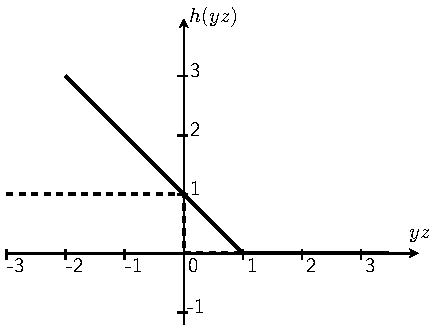
\includegraphics[width=8cm]{Chapters/09_SupportVectorMachines/20_softmarginsvm/latex/hinge.pdf}
    }
    % \myrule
\end{figure}
% ******************************************************************************


 
Ở đây, chúng ta làm quen với một hàm số khác cũng được sử dụng nhiều trong các hệ thống phân loại. Hàm số này có dạng 
\begin{equation*} 
J_n(\mathbf{w}, b) = \max(0, 1 - y_nz_n) 
\end{equation*} 
Hàm này có tên là \textit{mất mát bản lề} (hinge loss). Trong đó, $z_n = \bw^T\bx_n + b$ còn được gọi là \textit{điểm số} (score) của $\mathbf{x}_n$ ứng với cặp hệ số $(\mathbf{w},
b)$, $y_n = \pm 1$ là nhãn của $\bx_n$. Hình~\ref{fig:20_3} mô tả đồ thị hàm mất mát bản lề\footnote{Đồ thị của hàm số này có dạng chiếc bản lề.} $f(yz) = \max(0, 1 - yz)$ và
so sánh với hàm \textit{mất mát không-một}
({zero-one loss}). Hàm mất mát không-một trả về không nếu một điểm được phân loại đúng và trả về một nếu điểm đó bị phân loại sai. Như vậy, mất mát không-một là hàm {đếm số điểm bị
phân loại sai} của tập huấn luyện. Trong Hình~\ref{eqn:20_3}, biến số là $yz$ là tích của đầu ra
mong muốn $y$ và điểm số $z$. Những điểm ở phía phải của trục
tung ứng với những điểm được phân loại đúng, tức $z$ tìm được cùng dấu với $y$.
Những điểm ở phía trái của trục tung ứng với các điểm bị phân loại sai. Ta có
các nhận xét sau đây: 
\index{mất mát không-một -- zero-one loss}
\begin{itemize}
    \item Với mất mát không-một, các điểm dữ liệu có điểm số ngược dấu
    với đầu ra mong muốn ($yz < 0$) sẽ gây ra mất mát như nhau và đều bằng một, bất kể
    chúng ở gần hay xa đường ranh giới (trục tung). Đây là một hàm rời rạc, rất
    khó tối ưu và không giúp đo đếm sự hy sinh nếu một điểm nằm quá xa so với đường hỗ trợ.
     
    \item Với mất mát bản lề, những điểm nằm trong vùng an toàn ứng
    với $yz \geq 1$ sẽ không gây ra mất mát gì. Những điểm nằm giữa đường hỗ trợ của
    lớp tương ứng và đường ranh giới ứng với $0 < y < 1$ sẽ gây
    ra một mất mát nhỏ (nhỏ hơn một). Những điểm bị phân loại lỗi, tức $yz
    < 0$ sẽ gây ra mất mát lớn hơn. Vì vậy, khi tối thiểu hàm mất mát, ta sẽ
    hạn chế được những điểm bị phân loại lỗi và sang lớp kia quá nhiều. Đây chính là một ưu điểm của mất mát bản lề.
     
    \item Mất mát bản lề là một hàm liên tục, và \textit{có đạo hàm tại gần
    như mọi nơi} ({almost everywhere differentiable}) trừ điểm có hoành độ bằng 1. Ngoài ra, đạo hàm của hàm này theo $yz$ cũng rất dễ xác định: bằng -1 tại các điểm nhỏ hơn 1 và bằng 0 tại các điểm lớn hơn 1. Tại 1, ta có thể coi đạo hàm của nó bằng 0. 
\end{itemize}
 
 
\subsection{Xây dựng hàm mất mát}
Xét bài toán SVM lề mềm sử dụng
mất mát bản lề, với mỗi cặp $(\mathbf{w}, b)$, đặt
\begin{equation} 
L_n(\mathbf{w}, b) = \max(0, 1 - y_nz_n) = \max(0, 1 -
y_n(\mathbf{w}^T\mathbf{x}_n + b))
\end{equation}  
Lấy trung bình cộng của các mất mát này trên toàn tập huấn luyện ta được
\begin{equation*} 
L(\mathbf{w}, b) = \frac{1}{N}\sum_{n=1}^N L_n = \frac{1}{N}\sum_{n=1}^N \max(0,
1 - y_n(\mathbf{w}^T\mathbf{x}_n + b))
\end{equation*} 
% \textit{Câu hỏi đặt ra là, nếu ta trực tiếp tối ưu trung bình các hinge loss này thì
% điều gì sẽ xảy ra?}

Trong trường hợp dữ liệu hai lớp tách biệt tuyến tính,
giá trị tối ưu tìm được của $L(\mathbf{w}, b)$ sẽ bằng 0. Điều này nghĩa là:
\begin{equation} 
1 - y_n (\mathbf{w}^T\mathbf{x}_n + b) \leq 0, ~\forall n = 1, 2, \dots, N 
\end{equation} 
Nhân cả hai về với một hằng số $a > 1$ ta có:  
\begin{eqnarray}  
a - y_n (a\mathbf{w}^T\mathbf{x}_n + ab) &\leq& 0, ~\forall n = 1, 2, \dots, N \\\ 
\Rightarrow 1 - y_n (a\mathbf{w}^T\mathbf{x}_n + ab) &\leq& 1 - a < 0, ~\forall n = 1, 2, \dots, N 
\end{eqnarray} 

Điều này chỉ ra $(a\mathbf{w}, ab)$ cũng là nghiệm của bài toán. Nếu không có thêm ràng buộc, bài toán có thể dẫn tới nghiệm không ổn định vì $\bw$ và $b$ có thể lớn tuỳ ý!  
 
Để tránh hiện tượng này, chúng ta cần thêm một số hạng kiểm soát vào $L(\mathbf{w},
b)$ giống như cách làm để 
tránh quá khớp trong mạng neuron. Lúc này, ta sẽ có hàm mất mát
tổng cộng:
\begin{equation*} 
J(\mathbf{w}, b) = L(\mathbf{w}, b) + \lambda R(\mathbf{w}, b) 
\end{equation*} 
với $\lambda$ là một số dương, gọi là tham số kiểm soát, hàm
$R()$ giúp hạn chế việc các hệ số $(\mathbf{w}, b)$ quá lớn. Có nhiều
cách chọn hàm $R()$, nhưng cách phổ biến nhất là dùng chuẩn $\ell_2$, khi đó hàm mất mát của
SVM lề mềm trở thành:
\begin{equation} 
    \label{eqn:20_21}
    J(\mathbf{w}, b) = \frac{1}{N}\left(\underbrace{\sum_{n=1}^N \max(0, 1 -
        y_n(\mathbf{w}^T\mathbf{x}_n + b))}_{\text{mất mát bản lề}} +
        \underbrace{\frac{\lambda}{2}
        \|\mathbf{w}\|_2^2}_{\text{kiểm soát}}\right)
\end{equation} 
Kỹ thuật này tương đương với kỹ thuật suy giảm trọng số trong mạng neuron. Suy giảm trọng số không được áp dụng lên hệ số điều chỉnh $b$.
 
Ta thấy rằng hàm mất mát \eqref{eqn:20_21} tương đương hàm mất mát
\eqref{eqn:20_20} với $\lambda = \frac{1}{C}$. 
 
Trong phần tiếp theo của mục này, chúng ta sẽ quan tâm tới bài toán tối ưu hàm
mất mát được cho trong \eqref{eqn:20_21}. Trước hết, đây là một hàm lồi theo
$\bw, b$ vì các lý do sau: 
\begin{itemize}
    \item $1 - y_n(\bw^T\bx_n + b)$ là một hàm lồi vì nó tuyến tính theo $\bw, b$. Hàm lấy giá trị lớn hơn trong hai hàm lồi là một hàm lồi. Vì
    vậy, mất mát bản lề là một hàm lồi. 

    \item Chuẩn là một hàm lồi. 

    \item Tổng của hai hàm lồi là một hàm lồi. 

\end{itemize}
Vì hàm mất mát là lồi, các thuật toán gradient descent với tốc độ học phù hợp sẽ giúp tìm nghiệm của bài toán một cách hiệu quả. 

\subsection{Tối ưu hàm mất mát}
Để sử dụng gradient descent, chúng ta cần
tính đạo hàm của hàm mất mát theo $\bw$ và $b$. 

% \begin{equation}
%     \frac{\partial \frac{\lambda}{2}\|\bw\|_2^2}{\partial \bw} = \lambda
%     \bw;~\quad
%     \frac{\partial \frac{\lambda}{2}\|\bw\|_2^2}{\partial b} = 0 
% \end{equation}
Đạo hàm của mất mát bản lề không quá phức tạp:
\begin{eqnarray*}
    % \frac{\partial \max(0, 1 - y_n(\mathbf{w}^T\mathbf{x}_n + b))}{\partial \bw}
    \nabla_{\bw} \left(\max(0, 1 - y_n(\mathbf{w}^T\mathbf{x}_n + b))\right)
    &=& 
    \left\{ 
    \begin{matrix}
        -y_n\bx_n &~~\text{nếu}~~~ 1 - y_n(\bw^T\bx_n + b) \geq 0 \\
        \bzero &\text{o.w.}
    \end{matrix}
    \right. \\
    % \frac{\partial \max(0, 1 - y_n(\mathbf{w}^T\mathbf{x}_n + b))}{\partial b}
    \nabla_{b                                     } \left(\max(0, 1 -
    y_n(\mathbf{w}^T\mathbf{x}_n + b))\right)
    &=& 
    \left\{ 
    \begin{matrix}
        -y_n &~~~~~\text{nếu}~~~ 1 - y_n(\bw^T\bx_n + b) \geq 0 \\
        0 &\text{o.w.}
    \end{matrix}
    \right.  
\end{eqnarray*}
Phần kiểm soát cũng có đạo hàm tương đối đơn giản:
\begin{equation*}
    % \frac{\partial \frac{\lambda}{2}\|\bw\|_2^2}{\partial \bw} 
    \nabla_{\bw}\left(\frac{\lambda}{2}\|\bw\|_2^2\right)
    = \lambda
    \bw;~\quad
    \nabla_{b}\left(\frac{\lambda}{2}\|\bw\|_2^2\right)= 0 
\end{equation*}
% Nếu cập nhật bằng gradient descent thông qua chỉ một điểm dữ liệu $(\bx_n, y_n)$
% (\textit{stochastic gradient descent}). 
Khi sử dụng stochastic gradient descent trên từng điểm dữ liệu, nếu $ 1 - y_n(\mathbf{w}^T\mathbf{x}_n +
b) < 0$, ta không cần cập nhật và chuyển sang điểm tiếp theo. Ngược lại biểu
thức cập nhật cho $\bw, b$ được
cho bởi:
\begin{align*}
    &\bw \assign \bw - \eta (-y_n\bx_n + \lambda \bw); & b &\assign b + \eta
    y_n &&\text{nếu}& 1 - y_n(\mathbf{w}^T\mathbf{x}_n + b) \geq 0) \\
    &\bw \assign \bw -\eta \lambda \bw; & b &\assign b &&\text{o.w.}
\end{align*}
với $\eta$ là tốc độ học. 
Với {mini-batch gradient descent} hoặc {batch gradient descent},
các biểu thức đạo hàm trên đây hoàn toàn có thể được lập trình bằng các kỹ thuật
vector hóa như chúng ta sẽ thấy trong mục tiếp theo.

%  --  --  --  -- 
 
 
% Nhận thấy rằng ta có thể khiến biểu thức \eqref{eqn:20_19} gọn hơn một chút bằng
% cách sử dụng \textit{bias trick} như đã làm trong linear regression hay các
% chương về neural network. Bằng cách \textit{mở rộng} thêm một thành phần bằng 1
% vào các điểm dữ liệu $\mathbf{x}_n \in \mathbb{R}^d$ để được $\bar{\mathbf{x}}_n \in \mathbb{R}^{d+1}$ và kết hợp $\mathbf{w}, b$ thành một vector $\bar{\mathbf{w}} = [\mathbf{w}^T, b]^T \in \mathbb{R}^{d+1}$ ta sẽ có một biểu thức gọn hơn. Khi đó, hàm mất mát trong \eqref{eqn:20_21} có thể được viết gọn thành:
% \begin{equation} 
% J(\mathbf{\bar{w}}) = \underbrace{\sum_{n=1}^N \max(0, 1 - y_n\bar{\mathbf{w}}^T\mathbf{\bar{x}}_n)}_{\text{hinge loss}} + \underbrace{\frac{\lambda}{2} \|\mathbf{w}\|_2^2}_{\text{regularization}} 
% \end{equation} 
 
% Các bạn có thể nhận thấy rằng đây là một hàm lồi theo $\mathbf{\bar{w}}$ vì: 
 
% \begin{itemize}
% \item $1 - y_n\bar{\mathbf{w}}^T\mathbf{\bar{x}}_n$ là một hàm tuyến tính nên nó là một hàm lồi. Hàm hằng số là một hàm lồi, $\max$ cuả hai hàm lồi là một hàm lồi. Vậy biểu thức hinge loss là một hàm lồi.  
 
% \item Norm là một hàm lồi, vậy số hạng regularization cũng là một hàm lồi.  
 
% \item Tổng của hai hàm lồi là một hàm lồi.  
 
% Vì bài toán tối ưu bây giờ là không ràng buộc, chúng ta có thể sử dụng các phương pháp Gradient Descent để tối ưu. Hơn nữa, vì tính chất lồi của hàm mất mát, nếu chọn \textit{learning rate} không quá lớn và số vòng lặp đủ nhiều, thuật toán sẽ hội tụ tới điểm \textit{global optimal} của bài toán.  
% \end{itemize}
 
 
% \subsection{Tối ưu hàm mất mát }
% Trước hết ta cần tính được đạo hàm của hàm mất mát theo $\mathbf{\bar{w}}$. Việc này thoáng qua có vẻ hơi phức tạp vì ta cần tính đạo hàm của hàm $\max$, nhưng nếu chúng ta nhìn vào đạo hàm của hinge loss, ta có thể tính được đạo hàm theo $\mathbf{\bar{w}}$ một cách đơn giản.  
 
% Chúng ta tạm quên đi đạo hàm của phần regularization vì nó đơn giản bằng $\lambda \left[\begin{matrix} \mathbf{w}\\\ 0 \end{matrix}\right]$ với thành phần 0 ở cuối chính là đạo hàm theo bias của thành phần regularization. 
 
% Với phần hinge loss, xét từng điểm dữ liệu, ta có hai trường hợp:  

% \begin{itemize}
%     \item TH1: Nếu $ 1 - y_n \mathbf{\bar{w}}^T\mathbf{\bar{x}}_n \leq 0$, ta có ngay đạo hàm theo $\mathbf{\bar{w}}$ bằng 0.  
     
%     \item TH2: Nếu $ 1 - y_n \mathbf{\bar{w}}^T\mathbf{\bar{x}}_n > 0$, đạo hàm theo $\mathbf{w}$ chính là $-y_n\mathbf{x}_n$. 
% \end{itemize}
 
% Để tính gradient cho hàm mất mát trên toàn bộ dữ liệu, chúng ta cần một chút kỹ năng biến đổi đại số tuyến tính.  
 
 
% Đặt:  
% \begin{eqnarray}  
% \label{eqn:20_22}
%     \mathbf{Z} &=& [y_1 \mathbf{\bar{x}}_1, y_2 \mathbf{\bar{x}}_2, \dots, y_N\mathbf{\bar{x}}_N] \\\ 
% \label{eqn:20_23}
%     \mathbf{u} &=& [y_1\mathbf{\bar{w}}^T\mathbf{\bar{x}}_1,y_2\mathbf{\bar{w}}^T\mathbf{\bar{x}}_2, \dots, y_N \mathbf{\bar{w}}^T \mathbf{\bar{x}}_N] = \mathbf{\bar{w}}^T\mathbf{Z}   
% \end{eqnarray} 
 
% với chú ý rằng $\mathbf{u}$ là một vector hàng.  
 
% Tiếp tục, ta cần xác định các vị trí của $\mathbf{u}$ có giá trị nhỏ hơn 1, tức ứng với TH2 ở trên. Bằng cách đặt:  
% \begin{equation*} 
% \mathcal{H} = \{n: u_n < 1\} 
% \end{equation*} 
% ta có thể suy ra cách tính đạo hàm theo $\mathbf{\bar{w}}$ của hàm mất mát là: 

% \begin{equation} 
%     \label{eqn:20_24}
% % \begin{aligned}
%     \nabla J(\mathbf{\bar{w}}) = \sum_{n \in \mathcal{H}} - y_n\mathbf{\bar{x}}_n  + \lambda  
%     \left[\begin{matrix} \mathbf{w}\\\ 0 \end{matrix}\right]
% % \end{aligned}
% \end{equation} 

% Các bạn sẽ thấy cách tính toán giá trị này một cách hiệu quả trong phần lập trình.  
 
% Vậy quy tắc cập nhật của $\mathbf{\bar{w}}$ sẽ là:  
% \begin{equation} 
%     \label{eqn:20_25}
%     \mathbf{\bar{w}} = \mathbf{\bar{w}} - \eta \left(\sum_{n \in \mathcal{H}} - y_n\mathbf{\bar{x}}_n  + \lambda \left[\begin{matrix} \mathbf{w}\\\ 0 \end{matrix}\right]\right)
% \end{equation} 
% với $\eta$ là \textit{learning rate}. 
 
% Với các bài toán large-scale, ta có thể sử dụng phương pháp Mini-batch Gradient Descent để tối ưu. Đây chính là một ưu điểm của hướng tiếp cận theo hinge loss.  
 
\section{Lập trình với SVM lề mềm}
Trong mục này, nghiệm của một bài toán SVM lề mềm được tìm bằng ba cách khác nhau: sử dụng thư viện sklearn, giải bài toán đối ngẫu
bằng CVXOPT, và giải bài toán tối ưu không ràng buộc bằng gradient
descent. Giá trị $C$ được sử dụng là 100.
Nếu mọi tính toán từ đầu chương là chính xác, nghiệm của ba cách làm này sẽ
gần giống nhau, sự khác nhau có thể đến từ sai số tính toán.
Chúng ta cũng sẽ thay $C$ bởi những giá trị khác nhau và quan sát sự thay đổi của lề. 
 
% \subsection{Giải bài toán Soft Margin bằng 3 cách khác nhau}
 
% Source code cho phần này có thể được tìm thấy \href{https://github.com/tiepvupsu/tiepvupsu.github.io/blob/master/assets/20_softmarginsvm/plt/softmargin%20SVM%20Example.ipynb}{tại đây}. 
 
Khai báo thư viện và tạo dữ liệu giả:
 
\begin{lstlisting}[language=Python]
from __future__ import print_function
import numpy as np 
import matplotlib.pyplot as plt
np.random.seed(22)

means = [[2, 2], [4, 2]]
cov = [[.7, 0], [0, .7]]
N = 20 # number of samplers per class 
X0 = np.random.multivariate_normal(means[0], cov, N) # each row is a data point 
X1 = np.random.multivariate_normal(means[1], cov, N)
X = np.concatenate((X0, X1))
y = np.concatenate((np.ones(N), -np.ones(N)))
\end{lstlisting}

Hình \ref{fig:20_5} minh hoạ các điểm dữ liệu của hai lớp. Hai lớp dữ liệu gần tách biệt tuyến tính. 
 
% \begin{figure}[t]
%     % caption on side     
%     \floatbox[{\capbeside\thisfloatsetup{capbesideposition={right,top},capbesidewidth=6cm}}]{figure}[\FBwidth]
%     {\caption{ 
%     Tạo dữ liệu cho thí nghiệm. Dữ liệu của hai lớp là \textit{gần như linearly
%         separable}.
%     }
%     \label{fig:20_4}}
%     { % figure here
%     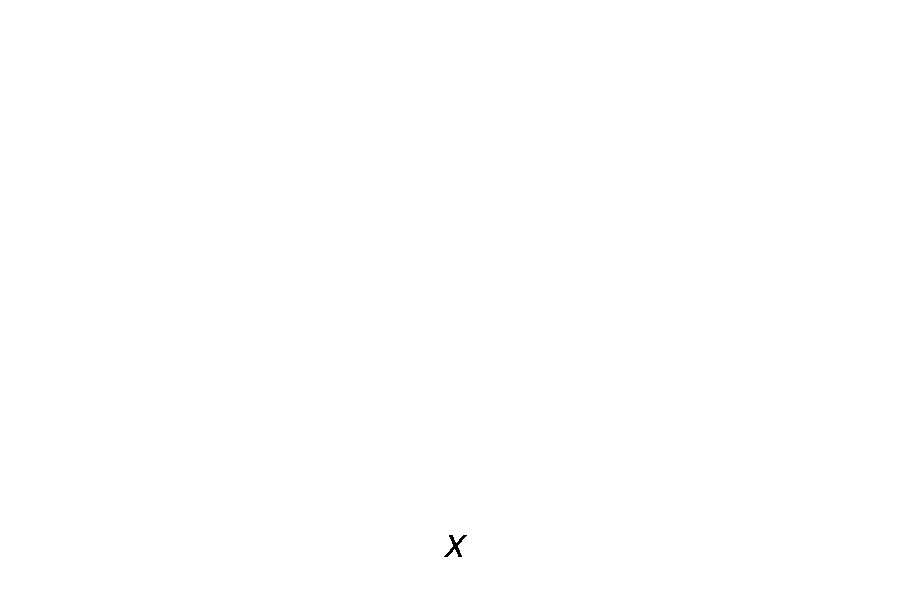
\includegraphics[width=.5\textwidth]{Chapters/09_SupportVectorMachines/20_softmarginsvm/plt/data.pdf}
%     }
%     % \myrule
% \end{figure}
 
% \textbf{Giải bài toán bằng thư viện sklearn}
\subsection{Giải bài toán bằng thư viện sklearn}

\begin{lstlisting}[language=Python]
from sklearn.svm import SVC 
C = 100 
clf = SVC(kernel = 'linear', C = C) 
clf.fit(X, y)  
w_sklearn = clf.coef_.reshape(-1, 1) 
b_sklearn = clf.intercept_[0] 
print(w_sklearn.T, b_sklearn) 
\end{lstlisting}
% \newpage
\kq
\begin{lstlisting}[language=Python]
w_sklearn =  [[-1.87461946 -1.80697358]]
b_sklearn =  8.49691190196
\end{lstlisting}
 
 
% \textbf{Tìm nghiệm bằng cách giải bài toán đối ngẫu }
\subsection{Tìm nghiệm bằng cách giải bài toán đối ngẫu }

Đoạn mã dưới đây tương tự với việc giải bài toán SVM lề cứng có thêm chặn trên của các nhân tử Lagrange:
 
\begin{lstlisting}[language=Python]
from cvxopt import matrix, solvers
# build K
V = np.concatenate((X0, -X1), axis = 0) # V[n,:] = y[n]*X[n]
K = matrix(V.dot(V.T))
p = matrix(-np.ones((2*N, 1)))
# build A, b, G, h 
G = matrix(np.vstack((-np.eye(2*N), np.eye(2*N))))
h = np.vstack((np.zeros((2*N, 1)), C*np.ones((2*N, 1))))
h = matrix(np.vstack((np.zeros((2*N, 1)), C*np.ones((2*N, 1)))))
A = matrix(y.reshape((-1, 2*N))) 
b = matrix(np.zeros((1, 1))) 
solvers.options['show_progress'] = False
sol = solvers.qp(K, p, G, h, A, b)

l = np.array(sol['x']).reshape(2*N) # lambda vector 

# support set 
S = np.where(l > 1e-5)[0] 
S2 = np.where(l < .999*C)[0]
# margin set 
M = [val for val in S if val in S2] # intersection of two lists

VS = V[S]           # shape (NS, d)
lS = l[S]           # shape (NS,)
w_dual = lS.dot(VS) # shape (d,)
yM = y[M]           # shape(NM,)
XM = X[M]           # shape(NM, d)
b_dual = np.mean(yM - XM.dot(w_dual)) # shape (1,)
print('w_dual = ', w_dual)
print('b_dual = ', b_dual)
\end{lstlisting}
\kq 
\begin{lstlisting}[language=Python]
w_dual =  [-1.87457279 -1.80695039]
b_dual =  8.49672109814
\end{lstlisting}


% \begin{lstlisting}[language=Python]
% lambda =  
%  [[  1.11381472e-06   9.99999967e+01   1.10533112e-06   6.70163540e-06 
%     3.40838760e+01   4.73972850e-06   9.99999978e+01   3.13320446e-06 
%     9.99999985e+01   5.06729333e+01   9.99999929e+01   3.23564235e-06 
%     9.99999984e+01   9.99999948e+01   1.37977626e-06   9.99997155e+01 
%     3.45005660e-06   1.46190314e-06   5.50601997e-06   1.45062544e-06 
%     1.85373848e-06   1.14181647e-06   8.47565685e+01   9.99999966e+01 
%     9.99999971e+01   8.00764708e-07   2.65537193e-06   1.45230729e-06 
%     4.15737085e-06   9.99999887e+01   9.99999761e+01   8.98414770e-07 
%     9.99999979e+01   1.75651607e-06   8.27947897e-07   1.04289116e-06 
%     9.99999969e+01   9.07920759e-07   8.83138295e-07   9.99999971e+01]] 
% \end{lstlisting}
 
% Trong các thành phần của \pythoninline{lambda} tìm được, có rất nhiều thành phần nhỏ tới \pythoninline{1e-6} hay \pythoninline{1e-7}. Đây chính là các \pythoninline{lambda_i = 0}. Có rất nhiều phần tử xấp xỉ \pythoninline{9.99e+01}, đây chính là các \pythoninline{lambda_i} bằng với \pythoninline{C = 100}, tương ứng với các support vectors không nằm trên margins, các sai số nhỏ xảy ra do tính toán. Các giá trị còn lại nằm giữa \pythoninline{0} và \pythoninline{100} là các giá trị tương ứng với các điểm nằm chính xác trên hai margins.  
 
% Tiếp theo, ta cần tính \pythoninline{w} và \pythoninline{b} theo công thức $(15)$ và $(16)$. Trước đó ta cần tìm tập hợp các điểm support và những điểm nằm trên margins.  
 
% \begin{lstlisting}[language=Python]
% S = np.where(l > 1e-5)[0] # support set  
% S2 = np.where(l < .999*C)[0]  
 
% M = [val for val in S if val in S2] # intersection of two lists 
 
% XT = X.T # we need each column to be one data point in this alg 
% VS = V[:, S] 
% lS = l[S] 
% yM = y[M] 
% XM = XT[:, M] 
 
% w_dual = VS.dot(lS).reshape(-1, 1) 
% b_dual = np.mean(yM.T - w_dual.T.dot(XM)) 
% print(w_dual.T, b_dual)  
% \end{lstlisting}
% Kết quả: 
% \begin{lstlisting}[language=Python]
% [[-1.87457279 -1.80695039]] 8.49672109815 
% \end{lstlisting}
 
Kết quả này gần giống với kết quả tìm được bằng sklearn. 

% \textbf{Tìm nghiệm bằng giải bài toán tối ưu không ràng buộc }
\subsection{Tìm nghiệm bằng giải bài toán tối ưu không ràng buộc }

Trong phương pháp này, chúng ta cần tính gradient của hàm mất mát. Như thường lệ, cần kiểm chứng tính chính xác của đạo hàm này. 
 Chú ý rằng trong phương pháp này, ta cần dùng tham số \pythoninline{lam = 1/C}.
Trước hết viết các hàm tính giá trị hàm mất mát và đạo hàm theo $\bw$ và $b$:
\newpage
\begin{lstlisting}[language=Python]
lam = 1./C 
def loss(X, y, w, b): 
    """
    X.shape = (2N, d), y.shape = (2N,), w.shape = (d,), b is a scalar 
    """
    z = X.dot(w) + b # shape (2N,)
    yz = y*z
    return (np.sum(np.maximum(0, 1 - yz)) + .5*lam*w.dot(w))/X.shape[0]

def grad(X, y, w, b):
    z = X.dot(w) + b # shape (2N,)
    yz = y*z         # element wise product, shape (2N,)
    active_set = np.where(yz <= 1)[0] # consider 1 - yz >= 0 only 
    _yX = - X*y[:, np.newaxis]   # each row is y_n*x_n 
    grad_w = (np.sum(_yX[active_set], axis = 0) + lam*w)/X.shape[0]
    grad_b = (-np.sum(y[active_set]))/X.shape[0]
    return (grad_w, grad_b)   

def num_grad(X, y, w, b):
    eps = 1e-10
    gw = np.zeros_like(w)
    gb = 0
    for i in xrange(len(w)):
        wp = w.copy()
        wm = w.copy()
        wp[i] += eps 
        wm[i] -= eps 
        gw[i] = (loss(X, y, wp, b) - loss(X, y, wm, b))/(2*eps)
    gb = (loss(X, y, w, b + eps) - loss(X, y, w, b - eps))/(2*eps)
    return (gw, gb) 

w = .1*np.random.randn(X.shape[1])
b = np.random.randn()
(gw0, gb0) = grad(X, y, w, b)
(gw1, gb1) = num_grad(X, y, w, b)
print('grad_w difference = ', np.linalg.norm(gw0 - gw1))
print('grad_b difference = ', np.linalg.norm(gb0 - gb1))
\end{lstlisting}
\kq
\begin{lstlisting}[language=Python]
grad_w difference =  1.27702840067e-06
grad_b difference =  4.13701854995e-08
\end{lstlisting}
Sự sai khác giữa hai cách tính gradient khá nhỏ; ta có thể tin tưởng sử dụng hàm
\pythoninline{grad} khi thực hiện gradient descent. 
\newpage
Đoạn mã dưới đây trình bày cách cập nhật nghiệm bằng gradient descent:
% ******************************************************************************
\begin{figure}[t]
    \begin{subfigure}{0.325\textwidth}
    % 
\includegraphics[width=\linewidth]{Chapters/09_SupportVectorMachines/20_softmarginsvm/plt/svm_sklearn.pdf}
    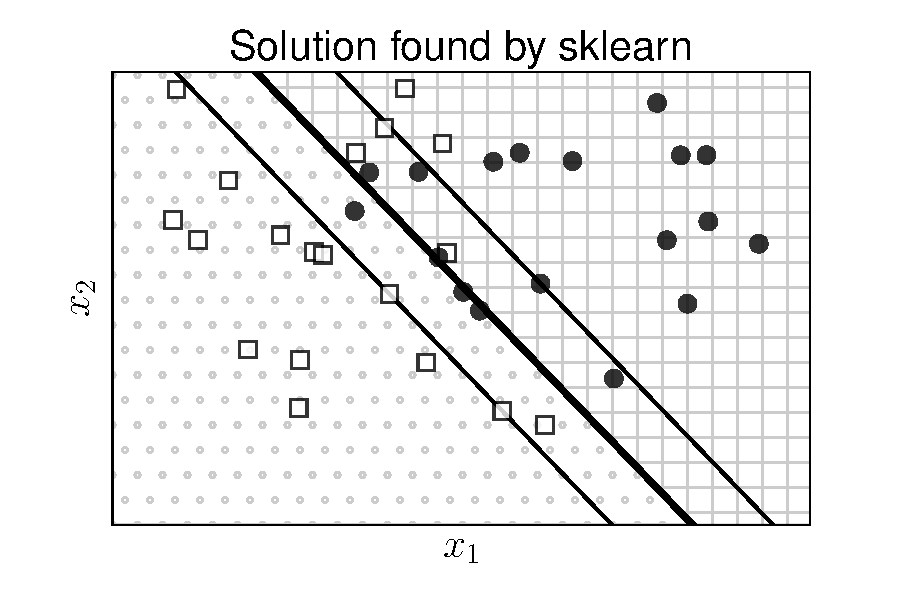
\includegraphics[width=\linewidth]{ebookML_src/src/softmargin_svm/svm_sklearn.pdf}
    \caption{}
    % \label{fig:subim1}
    \end{subfigure}
    \begin{subfigure}{0.325\textwidth}
    % 
\includegraphics[width=\linewidth]{Chapters/09_SupportVectorMachines/20_softmarginsvm/plt/svm_dual.pdf}
    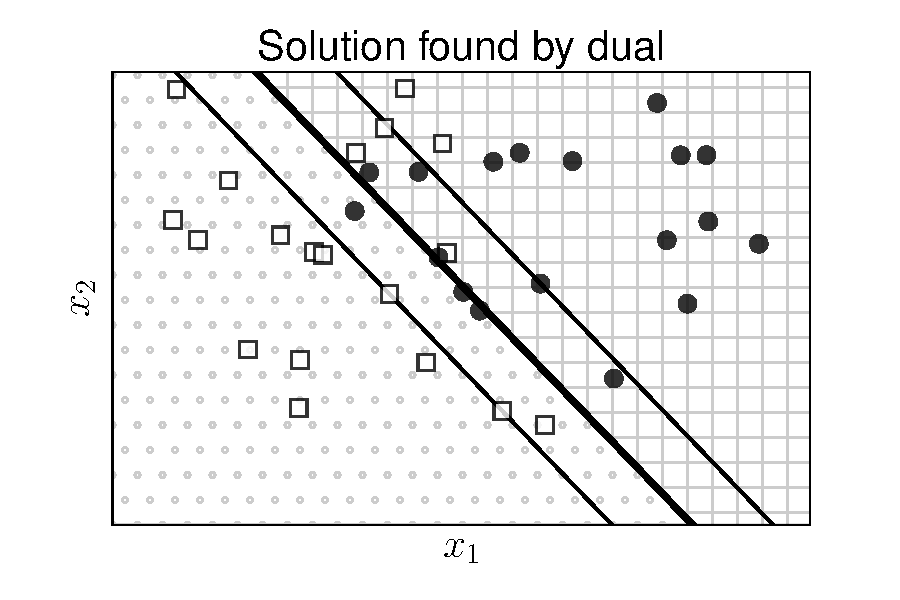
\includegraphics[width=\linewidth]{ebookML_src/src/softmargin_svm/svm_dual.pdf}
    \caption{}
    % \label{fig:subim2}
    \end{subfigure}
    \begin{subfigure}{0.325\textwidth}
    % 
\includegraphics[width=\linewidth]{Chapters/09_SupportVectorMachines/20_softmarginsvm/plt/svm_hinge.pdf}
    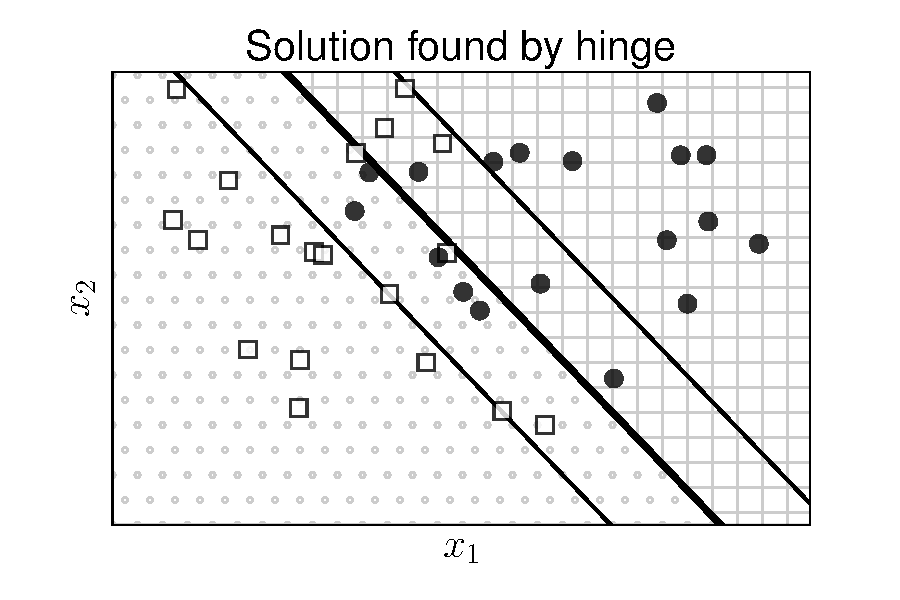
\includegraphics[width=\linewidth]{ebookML_src/src/softmargin_svm/svm_hinge.pdf}
    \caption{}
    % \label{fig:subim2}
    \end{subfigure}

    \caption{Các đường phân chia tìm được bởi ba cách khác nhau: a) Thư viện
    sklearn, b) Giải bài toán đối ngẫu bằng CVXOPT, c) Hàm mất mát bản lề. Các kết
    quả tìm được gần giống nhau.}
    \label{fig:20_5}
\end{figure}
% ******************************************************************************

% \newpage
\begin{lstlisting}[language=Python]
def softmarginSVM_gd(X, y, w0, b0, eta):
    w, b, it = w0, b0, 0     
    while it < 10000:
        it = it + 1
        (gw, gb) = grad(X, y, w, b)
        w -= eta*gw
        b -= eta*gb
        if (it % 1000) == 0:
            print('iter %d' %it + ' loss: %f' %loss(X, y, w, b))
    return (w, b)

w0 = .1*np.random.randn(X.shape[1]) 
b0 = .1*np.random.randn()
lr = 0.05
(w_hinge, b_hinge) = softmarginSVM_gd(X, y, w0, b0, lr)
print('w_hinge = ', w_dual)
print('b_hinge = ', b_dual)
\end{lstlisting}
% \newpage 
\kq 
\begin{lstlisting}
iter 1000 loss: 0.436460
iter 2000 loss: 0.405307
iter 3000 loss: 0.399860
iter 4000 loss: 0.395440
iter 5000 loss: 0.394562
iter 6000 loss: 0.393958
iter 7000 loss: 0.393805
iter 8000 loss: 0.393942
iter 9000 loss: 0.394005
iter 10000 loss: 0.393758
w_hinge =  [-1.87457279 -1.80695039]
b_hinge =  8.49672109814
\end{lstlisting}
Ta thấy rằng \pythoninline{loss} giảm dần và hội tụ theo thời gian. Nghiệm này cũng gần giống nghiệm tìm được bằng sklearn và CVXOPT. 
Hình~\ref{fig:20_5} mình hoạ các nghiệm tìm được bằng cả ba phương pháp.
Ta thấy rằng các nghiệm tìm được gần như giống nhau. 

 
% Trong thực hành, phương pháp 1 chắc chắn được lựa chọn. Hai phương pháp còn lại được dùng làm cơ sở cho các phương pháp SVM nâng cao hơn trong các bài sau.  
 
 
\subsection{Ảnh hưởng của $C$ lên nghiệm }

% ****************************************************************************** 
\begin{figure}[t]
    \begin{subfigure}{0.45\textwidth}
        % 
\includegraphics[width=0.95\linewidth]{Chapters/09_SupportVectorMachines/20_softmarginsvm/plt/ssvm5_01.pdf}
        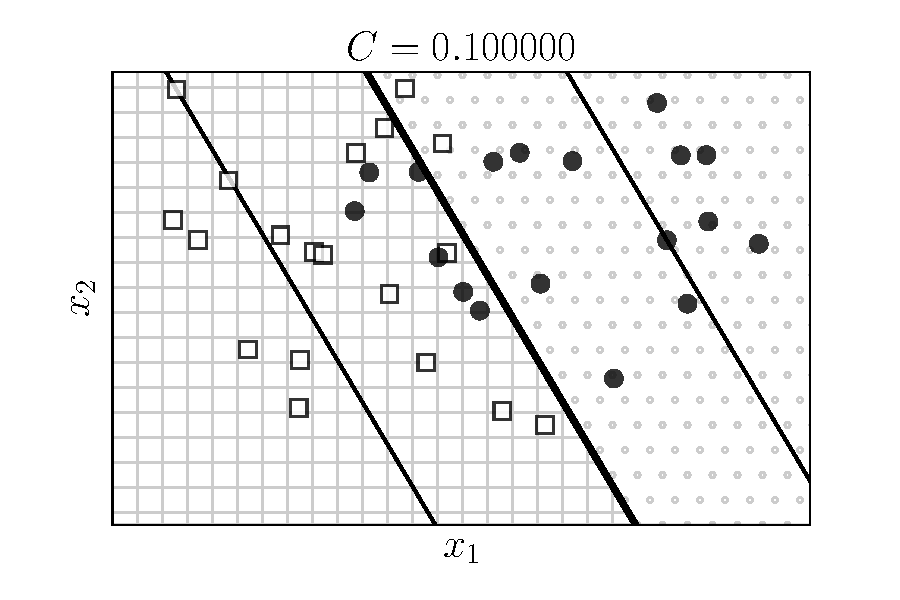
\includegraphics[width=0.95\linewidth]{ebookML_src/src/softmargin_svm/ssvm5_01.pdf}
    \end{subfigure}
    \begin{subfigure}{0.45\textwidth}
        % 
\includegraphics[width=0.95\linewidth]{Chapters/09_SupportVectorMachines/20_softmarginsvm/plt/ssvm5_1.pdf} 
        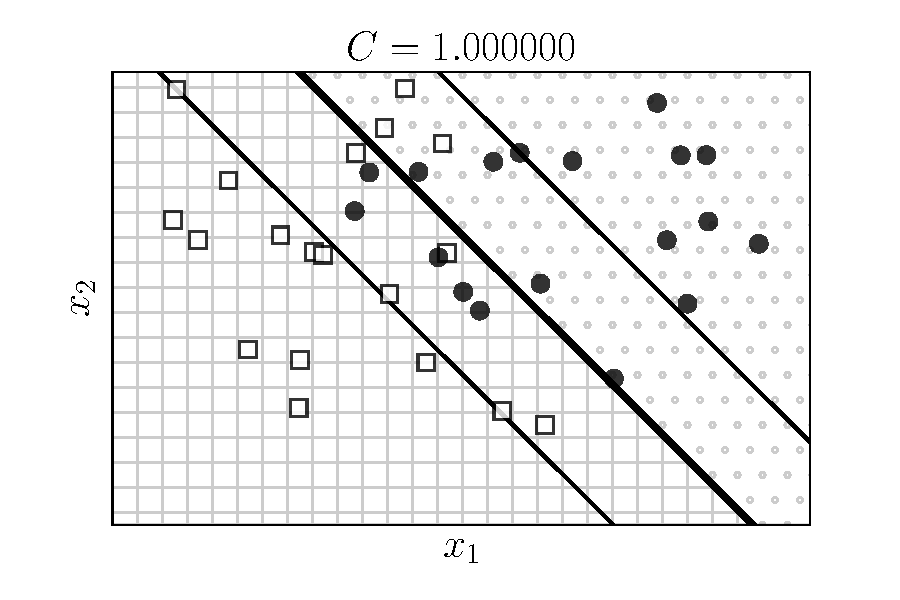
\includegraphics[width=0.95\linewidth]{ebookML_src/src/softmargin_svm/ssvm5_1.pdf}
    \end{subfigure}
    
    \begin{subfigure}{0.45\textwidth}
        % 
\includegraphics[width=0.95\linewidth]{Chapters/09_SupportVectorMachines/20_softmarginsvm/plt/ssvm5_10.pdf}
        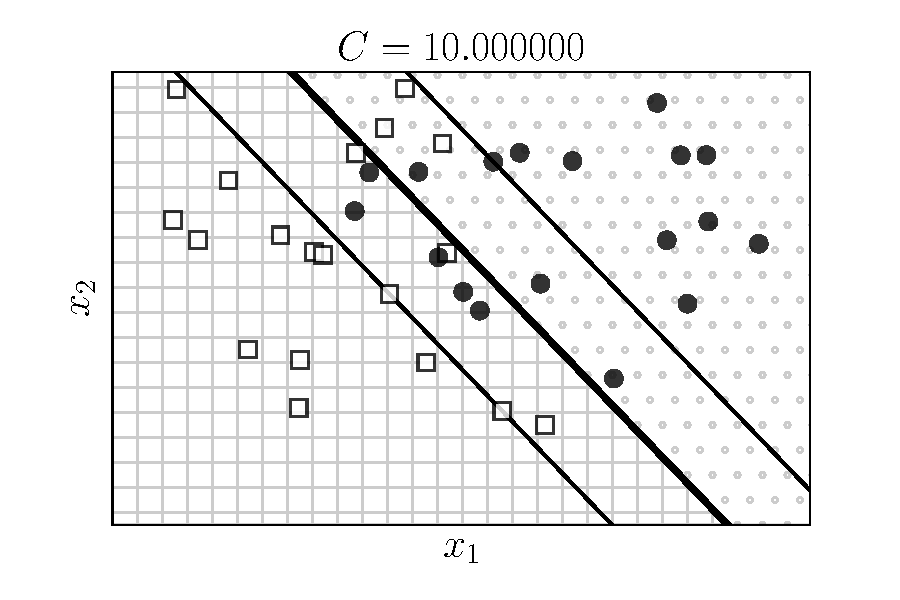
\includegraphics[width=0.95\linewidth]{ebookML_src/src/softmargin_svm/ssvm5_10.pdf}
    \end{subfigure}
    \begin{subfigure}{0.45\textwidth}
        % 
\includegraphics[width=0.95\linewidth]{Chapters/09_SupportVectorMachines/20_softmarginsvm/plt/ssvm5_100.pdf}
        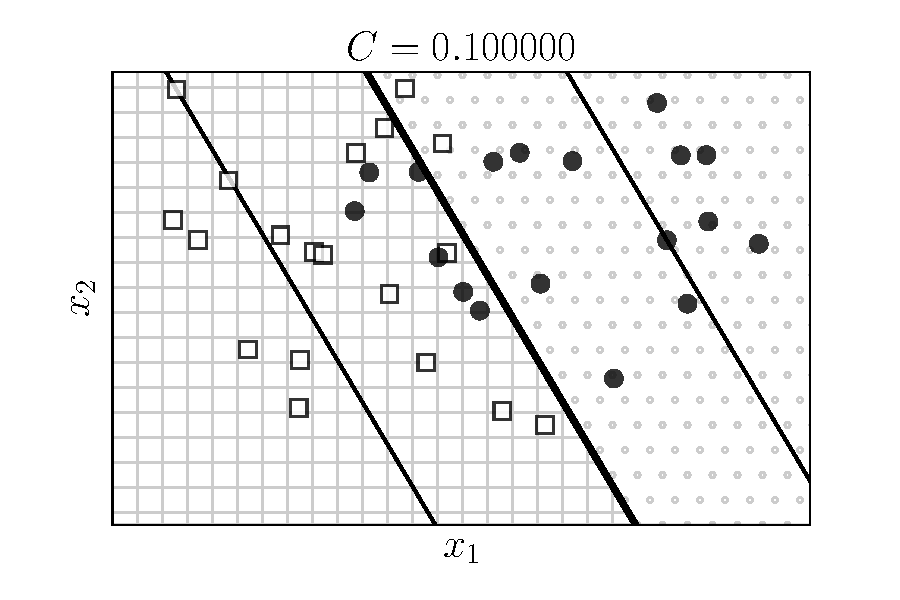
\includegraphics[width=0.95\linewidth]{ebookML_src/src/softmargin_svm/ssvm5_01.pdf}
    \end{subfigure}
    \caption{
    Ảnh hưởng của \(C\) lên nghiệm của SVM lề mềm. $C$ càng lớn thì biên
    càng nhỏ và ngược lại.
    }
    \label{fig:20_6}
\end{figure}
% ****************************************************************************** 
 
Hình~\ref{fig:20_6} minh hoạ nghiệm tìm được bằng sklearn với các giá trị $C$
khác nhau. Quan sát thấy khi $C$ càng lớn, biên càng nhỏ đi. Điều này phù hợp
với các suy luận ở đầu chương.
 
 
\section{Tóm tắt và thảo luận }
\begin{itemize}
    \item SVM thuần (SVM lề cứng) hoạt động không hiệu quả khi có nhiễu
    ở gần ranh giới hoặc khi dữ liệu giữa hai lớp gần tách biệt tuyến tính. SVM lề mềm có thể giúp khắc phục điểm này.  
     
    \item Trong SVM lề mềm, chúng ta chấp nhận lỗi xảy ra ở
    một
    vài điểm dữ liệu. Lỗi này được xác định bằng khoảng cách từ điểm đó tới
    đường hỗ trợ tương ứng. Bài toán tối ưu sẽ tối thiểu lỗi này bằng
    cách sử dụng thêm các biến lỏng lẻo. Có hai cách khác nhau giải bài toán tối ưu. 
     
    \item Cách thứ nhất là giải bài toán đối ngẫu. Bài toán đối ngẫu của
    SVM lề mềm rất giống với bài toán đối ngẫu của SVM lề cứng ngoại trừ việc có thêm ràng buộc chặn trên của các nhân tử Laggrange. Ràng buộc này còn được gọi là ràng buộc hộp. 
     
    \item Cách thứ hai là đưa bài toán về dạng không ràng buộc dựa trên mất mát bản lề. Trong phương pháp này, hàm mất mát thu được là một
    hàm lồi và có thể giải hiệu quả bằng các phương pháp gradient    descent.  
     
    \item SVM lề mềm yêu cầu chọn hằng số $C$. Hướng tiếp cận này còn được gọi là C-SVM. Ngoài ra, còn có một hướng tiếp cận khác cũng hay được sử dụng, gọi là
    $\nu$-SVM~\cite{scholkopf2000new}. 
     
    \item Mã nguồn trong chương này có thể được tìm thấy tại
    \url{https://goo.gl/PuWxba}. 
    
    \item LIBSVM là một thư viện SVM phổ biến  (\url{https://goo.gl/Dt7o7r}).
     
    \item {Đọc thêm:} L. Rosasco \etal,.
    {\textit{Are Loss
        Functions All the Same?}} (\url{https://goo.gl/QH2Cgr}). \textit{Neural
    Computation}.2004~\cite{rosasco2004loss}.
 \end{itemize} 
